\documentclass[10pt]{article}
\usepackage[a4paper,margin=2cm]{geometry}
\usepackage[T1]{fontenc}
\usepackage{mathptmx}
\usepackage[scaled=.9]{helvet}
\usepackage{amsmath,amssymb,graphicx,booktabs,xcolor,microtype,enumitem}
\usepackage[font=small,labelfont=bf]{caption}
\usepackage[hidelinks]{hyperref}
\usepackage{titlesec}
\titlespacing*{\section}{0pt}{8pt}{3pt}
\titlespacing*{\subsection}{0pt}{6pt}{2pt}
\titleformat{\section}{\normalfont\large\bfseries}{\thesection}{0.6em}{}
\setlist{nosep,leftmargin=1.2em}
\setlength{\parskip}{3pt}
\setlength{\parindent}{0pt}
\newcommand{\Device}{NVIDIA L40S}
\newcommand{\Backend}{torch}
\newcommand{\BackendNote}{All tiers run on real Tensor Cores via cuBLAS (PyTorch 2.14.1+cu130, CUDA 13.0).}
\newcommand{\Nq}{10}
\newcommand{\Ntraj}{65{,}536}
\newcommand{\Msteps}{200}
\newcommand{\Jterms}{19}
\newcommand{\Tevo}{2.0}
\newcommand{\SigmaVal}{0.129}
\newcommand{\StatErr}{5.0\times10^{-4}}
\newcommand{\Est}{+0.0258}
\newcommand{\BiasFp}{1.8\times10^{-9}}
\newcommand{\RmsFp}{2.6\times10^{-8}}
\newcommand{\MaxFp}{1.6\times10^{-7}}
\newcommand{\NstarFp}{5\times10^{15}}
\newcommand{\TimeFp}{4.4}
\newcommand{\BiasThree}{1.7\times10^{-8}}
\newcommand{\RmsThree}{4.5\times10^{-8}}
\newcommand{\MaxThree}{2.6\times10^{-7}}
\newcommand{\NstarThree}{6\times10^{13}}
\newcommand{\TimeThree}{6.1}
\newcommand{\BiasTf}{9.3\times10^{-7}}
\newcommand{\RmsTf}{1.3\times10^{-4}}
\newcommand{\MaxTf}{8.5\times10^{-4}}
\newcommand{\NstarTf}{2\times10^{10}}
\newcommand{\TimeTf}{2.7}
\newcommand{\BiasBf}{6.3\times10^{-5}}
\newcommand{\RmsBf}{1.7\times10^{-3}}
\newcommand{\MaxBf}{1.1\times10^{-2}}
\newcommand{\NstarBf}{4\times10^{6}}
\newcommand{\TimeBf}{2.4}
\newcommand{\BiasBfn}{2.9\times10^{-5}}
\newcommand{\RmsBfn}{1.1\times10^{-3}}
\newcommand{\MaxBfn}{7.0\times10^{-3}}
\newcommand{\NstarBfn}{2\times10^{7}}
\newcommand{\TimeBfn}{1.1}
\newcommand{\RatioTf}{138}
\newcommand{\TimeRef}{109.2}
\newcommand{\SingleFp}{38.85}
\newcommand{\LoopMinFp}{75}
\newcommand{\PadMinFp}{7}
\newcommand{\PadMaxFp}{57}
\newcommand{\SingleTf}{91.41}
\newcommand{\LoopMinTf}{61}
\newcommand{\PadMinTf}{6}
\newcommand{\PadMaxTf}{41}
\newcommand{\GapMin}{6}
\newcommand{\GapMax}{82}
\newcommand{\BenchDtwo}{2048}
\newcommand{\BenchJ}{19}
\newcommand{\BenchNmax}{65{,}536}
\newcommand{\CodeLine}{}


\begin{document}
{\Large\bfseries Is Tensor Core precision free?\par}
{\large Error-budgeted, grouped-GEMM simulation of randomized quantum trajectories\par}
\vspace{3pt}
{\small Avinash Singh, Fujitsu Research (Bangalore) \,·\, Prototype for Quantum Flywheel Track~2 (breaking quantum advantage claims) \,·\, October 2026\par}
\vspace{2pt}\hrule\vspace{6pt}

\textbf{Summary.} The proposal argues that classical refutations of advantage claims are limited by kernel engineering, and that low-precision Tensor Core arithmetic may cost nothing in physical accuracy because truncation and sampling errors dominate rounding error. This prototype tests the second claim on the smallest workload that carries both effects: a batched ensemble of randomized (qDRIFT) trajectories, where every time step is a set of GEMMs of multinomially skewed size. Running the \emph{same} \Ntraj{} sampled trajectories in five arithmetic tiers against an FP64 reference shows that TF32 adds a systematic error of $\BiasTf$ to the estimate, smaller than the statistical error until $N^\star\approx\NstarTf$ trajectories. BF16 crosses over at $N^\star\approx\NstarBf$, and FP32 or 3xTF32 at $N^\star\approx\NstarFp$. TF32 is also fast: the full ensemble ran in \TimeTf\,s against \TimeRef\,s for FP64 on the \Device. A timing study shows that standard ways of executing the skewed per-term GEMMs reach about 10\% of a single dense TF32 GEMM of equal work at small $N$, and \PadMinTf--\LoopMinTf\% at large $N$. This is the gap the proposed persistent grouped-GEMM kernel (K1) targets.

\section{Setup}
\textbf{Model and sampler.} Transverse-field Ising chain $H=-\sum_{i}Z_iZ_{i+1}-\sum_i X_i$ on $n=\Nq$ qubits ($J=\Jterms$ terms, $\lambda=\sum_j|h_j|$). qDRIFT draws $M=\Msteps$ terms i.i.d.\ with $p_j=|h_j|/\lambda$ and applies $e^{-i\tau\,\mathrm{sgn}(h_j)P_j}$ with $\tau=\lambda t/M$, $t=\Tevo$, starting from $|0\rangle^{\otimes n}$. Each trajectory $b$ yields $O_b=\tfrac1n\sum_i\langle\psi_b|Z_i|\psi_b\rangle$, and the estimator is $\hat O_N=\tfrac1N\sum_b O_b$ (here $\hat O_N=\Est$, $\sigma=\SigmaVal$).

\textbf{Grouped GEMM.} At step $k$ the trajectories are sorted by sampled term, so the step is one GEMM per term,
\[
\Psi_j \leftarrow \Psi_j\,R_j^{\!\top},\qquad \Psi_j\in\mathbb R^{m_j\times 2D},\qquad (m_1,\dots,m_J)\sim\mathrm{Multinomial}(N,p),
\]
with $R_j$ the real $2D\times2D$ form of $e^{-i\theta P_j}$ acting on $[\mathrm{Re}\,\psi,\mathrm{Im}\,\psi]$, $D=2^n$. Dense propagators are a deliberate GEMM-shaped stand-in for fused gate blocks and MPS-site contractions. They were verified against exact matrix exponentials to $10^{-15}$.

\textbf{Error budget.} For the estimate of $\langle O\rangle$,
\[
\bigl|\hat O_N-\langle O\rangle\bigr|\;\le\;\varepsilon_{\rm qDRIFT}(\tau,M)\;+\;\underbrace{\sigma/\sqrt N}_{\varepsilon_{\rm stat}}\;+\;\varepsilon_{\rm fp}.
\]
Every tier replays identical term sequences, so $\varepsilon_{\rm qDRIFT}$ is common and the paired differences $\delta_b=O_b^{\rm tier}-O_b^{\rm FP64}$ isolate arithmetic error. Their random part averages down as ${\rm rms}(\delta)/\sqrt N\ll\sigma/\sqrt N$, so the part that survives averaging is the bias $\beta=\mathbb E[\delta]$. A tier is \emph{free} while $|\beta|\le\sigma/\sqrt N$:
\[
N^\star=\bigl(\sigma/|\beta|\bigr)^2 .
\]
If $\beta$ is not resolved ($|\hat\beta|<2\,\mathrm{SE}$), $2\,\mathrm{SE}$ replaces $|\hat\beta|$ and $N^\star$ becomes a lower bound.

\textbf{Precision tiers.} FP32; 3xTF32 (operands split into TF32 high and low parts, three products); TF32 (10-bit mantissa inputs, FP32 accumulate); BF16 (7-bit mantissa inputs and state storage, FP32 accumulate), with and without per-step renormalization (which the trajectory unravelling performs anyway). Hardware for these results: \Device. \BackendNote

\section{Results}
\begin{figure}[h]
\centering
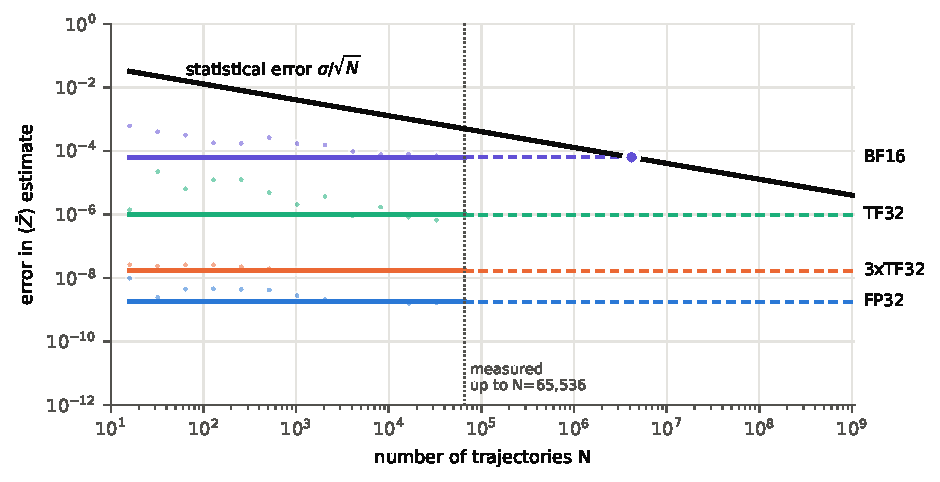
\includegraphics[width=0.86\linewidth]{fig_budget.pdf}
\caption{Error in the ensemble estimate of $\langle\bar Z\rangle$ against the number of trajectories $N$. Black: statistical error. Coloured lines: arithmetic bias $|\beta|$ of each tier, solid where measured and dashed where extrapolated; small dots show $|\bar\delta|$ on the first $N$ trajectories. A filled circle marks $N^\star$, where the tier stops being free.}
\label{fig:budget}
\end{figure}

\begin{table}[h]
\centering\small
\caption{Arithmetic error of each tier relative to FP64 on the same \Ntraj{} trajectories at $t=\Tevo$ (statistical error at this $N$: $\StatErr$). Run times are for the full ensemble on \Device; FP64 took \TimeRef\,s.}
\label{tab:tiers}
\begin{tabular}{lccccc}
\toprule
Tier & bias $|\beta|$ & rms$(\delta)$ & max$|\delta|$ & free up to $N^\star$ & time (s)\\
\midrule
FP32 & $\BiasFp$ & $\RmsFp$ & $\MaxFp$ & $\NstarFp$ & \TimeFp\\
3xTF32 & $\BiasThree$ & $\RmsThree$ & $\MaxThree$ & $\NstarThree$ & \TimeThree\\
TF32 & $\BiasTf$ & $\RmsTf$ & $\MaxTf$ & $\NstarTf$ & \TimeTf\\
BF16 & $\BiasBf$ & $\RmsBf$ & $\MaxBf$ & $\NstarBf$ & \TimeBf\\
BF16, no renorm. & $\BiasBfn$ & $\RmsBfn$ & $\MaxBfn$ & $\NstarBfn$ & \TimeBfn\\
\bottomrule
\end{tabular}
\end{table}

\begin{minipage}[t]{0.40\linewidth}\vspace{0pt}
\centering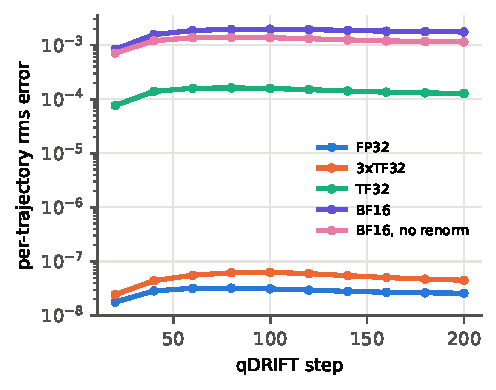
\includegraphics[width=\linewidth]{fig_depth.pdf}
\captionof{figure}{Per-trajectory rms error against circuit depth. It saturates instead of growing, because each step is unitary up to rounding and the state is renormalized.}
\label{fig:depth}
\end{minipage}\hfill
\begin{minipage}[t]{0.56\linewidth}\vspace{0pt}
\textbf{Findings.}
\begin{itemize}
\item \emph{TF32 is free for any realistic ensemble.} Its bias ($\BiasTf$) is ${\sim}$\RatioTf$\times$ below its per-trajectory rms error ($\RmsTf$): most rounding error cancels across trajectories. It meets the statistical error only at $N^\star\approx\NstarTf$, far beyond the $10^4$--$10^6$ trajectories a Gibbs-sampling estimate uses. It was also the fastest accurate tier (\TimeTf\,s vs.\ \TimeFp\,s FP32 and \TimeRef\,s FP64).
\item \emph{BF16 is free only for small ensembles} ($N^\star\approx\NstarBf$). A mixed-precision scheduler can use it for exploratory sweeps and switch to TF32 as $N$ grows.
\item \emph{3xTF32 is a safe FP32 substitute.} Its bias ($\BiasThree$) is larger than FP32's ($\BiasFp$) but still free up to $N^\star\approx\NstarThree$, so it can replace FP32 on Tensor Cores where FP64 is slow (Ada-class GPUs).
\item \emph{Error does not accumulate with depth} (Fig.~\ref{fig:depth}), which supports deep qDRIFT circuits at low precision.
\end{itemize}
\end{minipage}

\vspace{6pt}
\begin{figure}[h]
\centering
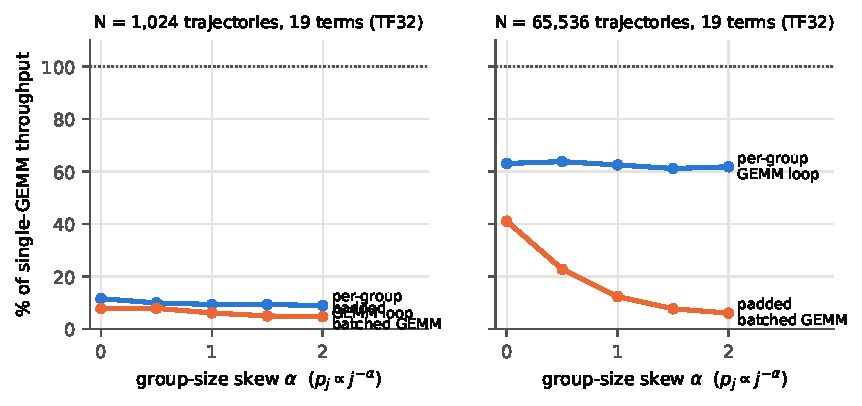
\includegraphics[width=0.92\linewidth]{fig_grouped.pdf}
\caption{Throughput of one trajectory step (\BenchJ{} skewed groups, $2D=\BenchDtwo$) as a fraction of a single dense GEMM doing the same useful work, against group-size skew. A per-group GEMM loop pays launch and scheduling overhead. Zero-padding to the largest group wastes $J\,m_{\max}/N$ of the work, which grows with skew. Hardware: \Device.}
\label{fig:grouped}
\end{figure}

\textbf{Grouping cost.} A single dense GEMM of this shape runs at \SingleTf\,TFLOP/s in TF32 (\SingleFp\,TFLOP/s in FP32). With $N=1{,}024$ trajectories, both standard paths stay near 10\% of that (Fig.~\ref{fig:grouped}, left): launch and scheduling overhead dominates. With $N=\BenchNmax$, the per-group loop reaches about \LoopMinTf\%, and padded batched GEMM falls from \PadMaxTf\% to \PadMinTf\% as the term distribution becomes skewed, the regime real Hamiltonians produce because $p_j\propto|h_j|$. Neither standard option reaches dense-GEMM throughput. A persistent grouped-GEMM kernel with size-aware tile scheduling (K1) is designed to close this gap, and the same kernel serves skewed symmetry sectors in tensor networks.

\IfFileExists{bq.tex}{\input{bq.tex}}{}

\section{How AI agents were used}
The prototype was built in one working session with an AI coding and research agent (Claude). The researcher set the scientific question (is the K3 hypothesis true for trajectory estimators?) and reviewed design choices. The agent then:
(i) turned the question into a falsifiable measurement, with paired differences over shared random sequences and the crossover $N^\star$;
(ii) wrote the simulator with interchangeable NumPy (CPU, bit-exact TF32/BF16 operand rounding) and PyTorch (CUDA Tensor Core) backends;
(iii) checked the propagators against exact matrix exponentials before any measurement;
(iv) ran a CPU validation sweep and packaged the GPU pipeline, which the researcher then ran on the \Device{} (smoke test against the CPU path first, then the full sweep and grouped-GEMM timing);
(v) produced every figure, table and number in this report directly from the result files, so a rerun on new hardware regenerates the document unchanged.
The same loop (question, validation, sweep, report) is how the funded project would run its experiments at scale on EC2 GPUs and IBM QPUs.

\section{What this means for the proposal, and next steps}
\begin{itemize}
\item \textbf{First target claim:} Floquet Ising prethermal dynamics on IBM Heron r3, up to 74 qubits (Leviatan et al., arXiv:2607.24937), where tensor networks did not converge and sparse Pauli-path runs on Fugaku stayed truncation-dependent. It is the same transverse-field Ising family as this prototype and an active candidate on the community Quantum Advantage Tracker.
\item \textbf{K3 (precision tiers):} the hypothesis holds for trajectory estimators. The scheduler can safely choose TF32 by default, and $N^\star$ gives a quantitative rule for when to move up a tier. Next: repeat for tensor-network truncation error, using the bond-dimension discarded weight in place of $\sigma/\sqrt N$.
\item \textbf{K1 (grouped GEMM):} the measured gap between per-group and dense execution is the target. Next: a persistent CUTLASS/CuTe kernel over skewed groups, benchmarked on this harness.
\item \textbf{K4 (trajectory engine):} extend from qDRIFT to unravelled KMS-detailed-balance Lindbladians (Chen--Li--Lu--Ying, arXiv:2407.06594), where jump sampling produces the same multinomial grouping, then scale to MPS trajectories for systems beyond statevector size.
\end{itemize}
\CodeLine

\end{document}
